% Options for packages loaded elsewhere
\PassOptionsToPackage{unicode}{hyperref}
\PassOptionsToPackage{hyphens}{url}
%
\documentclass[
]{book}
\usepackage{amsmath,amssymb}
\usepackage{iftex}
\ifPDFTeX
  \usepackage[T1]{fontenc}
  \usepackage[utf8]{inputenc}
  \usepackage{textcomp} % provide euro and other symbols
\else % if luatex or xetex
  \usepackage{unicode-math} % this also loads fontspec
  \defaultfontfeatures{Scale=MatchLowercase}
  \defaultfontfeatures[\rmfamily]{Ligatures=TeX,Scale=1}
\fi
\usepackage{lmodern}
\ifPDFTeX\else
  % xetex/luatex font selection
\fi
% Use upquote if available, for straight quotes in verbatim environments
\IfFileExists{upquote.sty}{\usepackage{upquote}}{}
\IfFileExists{microtype.sty}{% use microtype if available
  \usepackage[]{microtype}
  \UseMicrotypeSet[protrusion]{basicmath} % disable protrusion for tt fonts
}{}
\makeatletter
\@ifundefined{KOMAClassName}{% if non-KOMA class
  \IfFileExists{parskip.sty}{%
    \usepackage{parskip}
  }{% else
    \setlength{\parindent}{0pt}
    \setlength{\parskip}{6pt plus 2pt minus 1pt}}
}{% if KOMA class
  \KOMAoptions{parskip=half}}
\makeatother
\usepackage{xcolor}
\usepackage{longtable,booktabs,array}
\usepackage{calc} % for calculating minipage widths
% Correct order of tables after \paragraph or \subparagraph
\usepackage{etoolbox}
\makeatletter
\patchcmd\longtable{\par}{\if@noskipsec\mbox{}\fi\par}{}{}
\makeatother
% Allow footnotes in longtable head/foot
\IfFileExists{footnotehyper.sty}{\usepackage{footnotehyper}}{\usepackage{footnote}}
\makesavenoteenv{longtable}
\usepackage{graphicx}
\makeatletter
\newsavebox\pandoc@box
\newcommand*\pandocbounded[1]{% scales image to fit in text height/width
  \sbox\pandoc@box{#1}%
  \Gscale@div\@tempa{\textheight}{\dimexpr\ht\pandoc@box+\dp\pandoc@box\relax}%
  \Gscale@div\@tempb{\linewidth}{\wd\pandoc@box}%
  \ifdim\@tempb\p@<\@tempa\p@\let\@tempa\@tempb\fi% select the smaller of both
  \ifdim\@tempa\p@<\p@\scalebox{\@tempa}{\usebox\pandoc@box}%
  \else\usebox{\pandoc@box}%
  \fi%
}
% Set default figure placement to htbp
\def\fps@figure{htbp}
\makeatother
\setlength{\emergencystretch}{3em} % prevent overfull lines
\providecommand{\tightlist}{%
  \setlength{\itemsep}{0pt}\setlength{\parskip}{0pt}}
\setcounter{secnumdepth}{5}
\usepackage{booktabs}
\usepackage[]{natbib}
\bibliographystyle{plainnat}
\usepackage{bookmark}
\IfFileExists{xurl.sty}{\usepackage{xurl}}{} % add URL line breaks if available
\urlstyle{same}
\hypersetup{
  pdftitle={Quality Control Pipeline for Massively Parallel Reporter Assays (MPRAs)},
  pdfauthor={Omer Ronen},
  hidelinks,
  pdfcreator={LaTeX via pandoc}}

\title{Quality Control Pipeline for Massively Parallel Reporter Assays (MPRAs)}
\author{Omer Ronen}
\date{2025-12-28}

\begin{document}
\maketitle

{
\setcounter{tocdepth}{1}
\tableofcontents
}
\chapter*{Overview}\label{overview}
\addcontentsline{toc}{chapter}{Overview}

This pipeline is designed to help investigators evaluate the quality of their MPRA, quickly identify pitfalls, trace them to their source, and mitigate them. The scripts provided help ensure that the resulting MPRA data are suitable for robust statistical analysis and meaningful biological interpretation.
This Bookdown accompanies our guide for best practices for MPRAs, which outlines recommendations for study design and interpretation {[}REF{]}. The manuscript covers all key experimental and analytical steps, including library design, and estimation of activity differential activity. It then describes core problems that often compromise MPRA quality, illustrating how these issues manifest in the data, and offering practical strategies for correction and optimization.
Because each issue can influence multiple quality metrics, and each metric may be affected by several issues, the relationships form a many-to-many network. The figures presented below map these interdependencies and connect them to recommended diagnostic analyses.

\section*{Usage}\label{usage}
\addcontentsline{toc}{section}{Usage}

\pandocbounded{\includegraphics[keepaspectratio]{associations_root.png}}
A scheme of root problems, the impacted quality metrics and analyses for the cCRE-barcode association step.

\pandocbounded{\includegraphics[keepaspectratio]{activity_root.png}}
Root problems, impacted quality metrics and recommended analyses for the RNA and DNA quantification step.

The quality control (QC) pipeline is organized into three chapters:

\begin{itemize}
\tightlist
\item
  \begin{enumerate}
  \def\labelenumi{(\roman{enumi})}
  \tightlist
  \item
    QC of the barcode association step\\
  \end{enumerate}
\item
  \begin{enumerate}
  \def\labelenumi{(\roman{enumi})}
  \setcounter{enumi}{1}
  \tightlist
  \item
    QC of activity estimation\\
  \end{enumerate}
\item
  \begin{enumerate}
  \def\labelenumi{(\roman{enumi})}
  \setcounter{enumi}{2}
  \tightlist
  \item
    QC of differential activity estimation
  \end{enumerate}
\end{itemize}

For each analysis, we provide an example of a successful and an unsuccessful dataset to illustrate how they manifest in the analysis.

We welcome questions, feedback, or suggestions. Please feel free to reach out at david.gokhman {[}at{]} weizmann.ac.il.

\section*{Scripts}\label{scripts}
\addcontentsline{toc}{section}{Scripts}

All of these analyses are integrated into the quality control pipeline described in this resource, with scripts provided here: {[}link{]}.

\chapter{A guide for running the analyses notebook}\label{a-guide-for-running-the-analyses-notebook}

The QC pipeline has three main parts: Associations, Activity and Differential activity.
For each part, there is a jupyter notebook file that enables you to run all the analyses that are presented in this book.
Here we explain how to run these notebook files and what are the required inputs

\section{Associations}\label{associations}

First

\subsection{Input}\label{input}

Input files

\section{Activity}\label{activity}

Second

\subsection{Input}\label{input-1}

Input files

\section{Differential Activity}\label{differential-activity}

Third

\subsection{Input}\label{input-2}

Input files

\chapter{Associations QC}\label{associations-qc}

\section{BCs per cCRE}\label{bcs-per-ccre}

\textbf{Goal: An empirical cumulative function (eCDF) of BCs per cCRE}
\textbf{Input file: BC-cCRE association file}
\textbf{Evaluated metrics: BC replicability}

\includegraphics[width=0.49\linewidth]{external_figures/Max_MPRA_run2/Barcodes_per_cCRE} \includegraphics[width=0.49\linewidth]{external_figures/PMID_38766054_Reilly/Barcodes_per_cCRE}

\textbf{Legend:}
\textbf{Interpretation:}

\section{PCR bias - GC}\label{pcr-bias---gc}

\textbf{Goal: This analysis assesses GC content bias in PCR amplification}
\textbf{Input file: BC-cCRE association file}
\textbf{Evaluated metrics: Complexity}

\includegraphics[width=0.49\linewidth]{external_figures/Max_MPRA_run2/PCR_bias_GC} \includegraphics[width=0.49\linewidth]{external_figures/PMID_38766054_Reilly/PCR_bias_GC}

\textbf{Legend:}
\textbf{Interpretation: The successful example shows a relatively consistent number of reads per GC content, and PCR conditions that are optimized for the GC content levels of most cCREs (peaks are close to one another). The unsuccessful example shows both a strong amplification bias and suboptimal PCR conditions for the GC content levels of most cCREs}

\section{PCR bias - G Stretches}\label{pcr-bias---g-stretches}

\textbf{Goal: This analysis assesses G-stretches bias in PCR amplification}
\textbf{Input file: BC-cCRE association file}
\textbf{Evaluated metrics: Complexity}

\includegraphics[width=0.49\linewidth]{external_figures/placeholder} 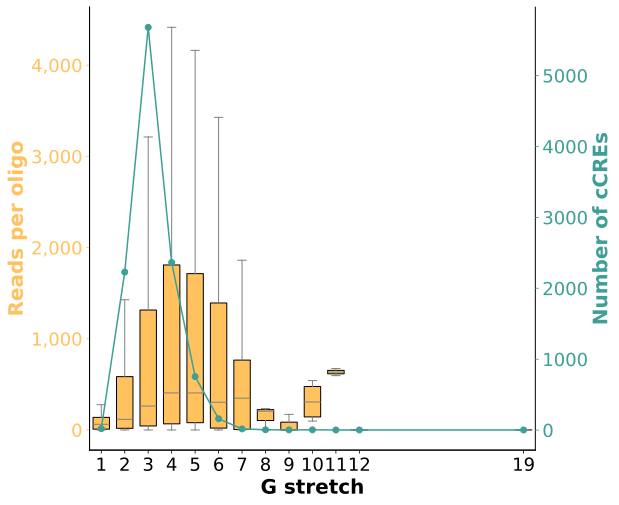
\includegraphics[width=0.49\linewidth]{external_figures/thylacine_biorxiv_Gallego_Romero/PCR_bias_G-stretches}

\textbf{Legend:}
\textbf{Interpretation:}

\section{UMIs per association}\label{umis-per-association}

\textbf{Goal:}
\textbf{Input file: Associations file before filtering for minimal number of associations}
\textbf{Evaluated metrics}:

\includegraphics[width=0.49\linewidth]{external_figures/Max_MPRA_run2/UMIs_per_association} \includegraphics[width=0.49\linewidth]{external_figures/PMID_38766054_Reilly/UMIs_per_association}

\textbf{Legend:}
\textbf{Interpretation:}

\section{Retained cCREs}\label{retained-ccres}

\textbf{Goal: Retained cCREs per increasing cutoffs of BC number per cCRE}
\textbf{Input file: BC-cCRE association file}
\textbf{Evaluated metrics: BC replicability}

\includegraphics[width=0.49\linewidth]{external_figures/Max_MPRA_run2/Retained_cCREs} \includegraphics[width=0.49\linewidth]{external_figures/PMID_38766054_Reilly/Retained_cCREs}

\textbf{Legend:}
\textbf{Interpretation:}

\section{cCREs per BC}\label{ccres-per-bc}

\textbf{Goal:}
\textbf{Input file: Associations file before filtering for BC promiscuity}
\textbf{Evaluated metrics: BC promiscuity}

\includegraphics[width=0.49\linewidth]{external_figures/Max_MPRA_run2/cCREs_per_BC_shuffled} \includegraphics[width=0.49\linewidth]{external_figures/PMID_38766054_Reilly/cCREs_per_BC}

\textbf{Legend:}
\textbf{Interpretation:}

\section{cCRE retention by sequencing depth}\label{ccre-retention-by-sequencing-depth}

\textbf{Goal: This analysis uses downsampling of sequencing reads to assess whether sequencing depth is sufficient}
\textbf{Input file: Downsampling association files}
\textbf{Evaluated metrics: complexity}

\includegraphics[width=0.49\linewidth]{external_figures/Max_MPRA_run2/Downsampling_Retained_cCREs} \includegraphics[width=0.49\linewidth]{external_figures/L3a2_281122/Downsampling_Retained_cCREs}

\textbf{Legend:}
\textbf{Interpretation:}

\section{BCs per cCRE by sequencing depth}\label{bcs-per-ccre-by-sequencing-depth}

\textbf{Goal: }
\textbf{Input file: Input file: Downsampling association files
}Evaluated metrics: Complexity**

\includegraphics[width=0.49\linewidth]{external_figures/L3a2_281122/Downsampling_Barcodes_per_cCRE} \includegraphics[width=0.49\linewidth]{external_figures/Max_MPRA_run2/Downsampling_Barcodes_per_cCRE}

\textbf{Legend:}
\textbf{Interpretation:}

\chapter{Activity QC}\label{activity-qc}

\subsection{Retained cCREs and barcodes}\label{retained-ccres-and-barcodes}

\textbf{Goal: Estimate the percentages of barcodes and cCREs retained after association}
\textbf{Input file: activity\_per\_rep}
\textbf{Evaluated metrics: final library complexity}:

\begin{verbatim}
## Good example: PMID_38766054_Reilly 
## Bad example: Max_MPRA_run2
\end{verbatim}

\pandocbounded{\includegraphics[keepaspectratio]{12-only_figs_activity_files/figure-latex/unnamed-chunk-3-1.pdf}}
\textbf{Legend:}
\textbf{Interpretation:}

\section{Activity distribution}\label{activity-distribution}

\textbf{Goal: Inferring tht power of the quantification step in determining activity}
\textbf{Input file: quantification table (comb\_df)}
\textbf{Evaluated metrics: activity dynamic range, noise, and statistical power}:

\begin{verbatim}
## Good example: PMID_38766054_Reilly 
## Bad example: humanMPRA_L4a2 
## Bad example 2: humanMPRA_L1a1_Neurons
\end{verbatim}

\pandocbounded{\includegraphics[keepaspectratio]{12-only_figs_activity_files/figure-latex/unnamed-chunk-4-1.pdf}}

\begin{verbatim}
## [1] "add arrows that indicate right tail, symmetry, or no activity detected"
\end{verbatim}

\textbf{Legend:}
\textbf{Interpretation:}

\section{P-value distribution}\label{p-value-distribution}

\textbf{Goal: Inferring the power of the statistical test}
\textbf{Input file: quantification table (comb\_df)}
\textbf{Evaluated metrics: ajusted P-value}:

Problem: nothitng looks mildly bad, max looks too bad.

\begin{verbatim}
## Good example: PMID_38766054_Reilly 
## Bad example: Max_MPRA_run2
\end{verbatim}

\pandocbounded{\includegraphics[keepaspectratio]{12-only_figs_activity_files/figure-latex/unnamed-chunk-5-1.pdf}}
\textbf{Legend:}
\textbf{Interpretation:}

\section{Downsampling analysis - active cCREs}\label{downsampling-analysis---active-ccres}

\textbf{Goal:}
\textbf{Input file:}
\textbf{Evaluated metrics}:

\pandocbounded{\includegraphics[keepaspectratio]{12-only_figs_activity_files/figure-latex/unnamed-chunk-6-1.pdf}}
\textbf{Legend:}
\textbf{Interpretation:}

\section{Cumulative RNA reads}\label{cumulative-rna-reads}

\textbf{Goal: To assess jackpotting}
\textbf{Input file: quantification table (comb\_df)}
\textbf{Evaluated metrics: DNA and RNA read counts}:

\begin{verbatim}
## Good example: PMID_38766054_Reilly 
## Bad example: d2Osteoblast_spiking_oligos
\end{verbatim}

\pandocbounded{\includegraphics[keepaspectratio]{12-only_figs_activity_files/figure-latex/unnamed-chunk-7-1.pdf}}
\textbf{Legend:}
\textbf{Interpretation:}

\section{Activity by sequencing depth}\label{activity-by-sequencing-depth}

\textbf{Goal: This analysis uses downsampling of sequencing reads to assess if sequencing depth is sufficient}
\textbf{Input file: Activity down sampling files}
\textbf{Evaluated metrics: RNA and DNA complexity}

\includegraphics[width=0.49\linewidth]{external_figures/modern_humanMPRA_Hob/Activity_by_sequencing_depth} \includegraphics[width=0.49\linewidth]{external_figures/modern_humanMPRA_NPC/Activity_by_sequencing_depth}

\textbf{Legend:}
\textbf{Interpretation:}

\section{Similarity between samples (PCA)}\label{similarity-between-samples-pca}

\textbf{Goal: to assess reproducibility between samples}
\textbf{Input file: cDNA\_reads\_by\_cell\_type}
\textbf{Evaluated metrics: sample clustering based on expression}:

mention in the bookdown: the importance of the percentage explained by the 1st and 2nd PCs.

\begin{verbatim}
## Good example: PMID_38766054_Reilly 
## Bad example: thylacine_biorxiv_Gallego_Romero
\end{verbatim}

\pandocbounded{\includegraphics[keepaspectratio]{12-only_figs_activity_files/figure-latex/unnamed-chunk-9-1.pdf}}
\textbf{Legend:}
\textbf{Interpretation:}

\section{Correlation between replicates}\label{correlation-between-replicates}

\textbf{Goal: To assess reproducibility between replicates}
\textbf{Input file: activity\_per\_rep}
\textbf{Evaluated metrics: correlation of expression between replicates}:

\begin{verbatim}
## Good example: thylacine_biorxiv_Gallego_Romero 
## Bad example: humanMPRA_L4a2
\end{verbatim}

\pandocbounded{\includegraphics[keepaspectratio]{12-only_figs_activity_files/figure-latex/unnamed-chunk-10-1.pdf}}

\begin{verbatim}
## Warning in rm(good_example_MPRA, bad_example_MPRA, bad_example_MPRA_2,
## analysis_name): object 'bad_example_MPRA_2' not found
\end{verbatim}

\textbf{Legend:}
\textbf{Interpretation:}

\section{Variation at various activity levels}\label{variation-at-various-activity-levels}

\textbf{Goal:}
\textbf{Input file:}
\textbf{Evaluated metrics}:

Omer is in charge of this part.

\begin{verbatim}
## Good example: PMID_38766054_Reilly 
## Bad example: humanMPRA_L4a2
\end{verbatim}

\pandocbounded{\includegraphics[keepaspectratio]{12-only_figs_activity_files/figure-latex/unnamed-chunk-11-1.pdf}}
\textbf{Legend:}
\textbf{Interpretation:}

\section{Correlation between replicates (controls)}\label{correlation-between-replicates-controls}

\textbf{Goal:}
\textbf{Input file: quantification table (comb\_df)}
\textbf{Evaluated metrics}:

\begin{verbatim}
## Good example: PMID_38766054_Reilly 
## Bad example: Max_MPRA_run2
\end{verbatim}

\pandocbounded{\includegraphics[keepaspectratio]{12-only_figs_activity_files/figure-latex/unnamed-chunk-12-1.pdf}}
\textbf{Legend:}
\textbf{Interpretation:}

\section{RNA\_DNA\_ratio}\label{rna_dna_ratio}

\textbf{Goal:}
\textbf{Input file:}
\textbf{Evaluated metrics}:

\begin{verbatim}
## Good example: PMID_38766054_Reilly 
## Bad example: humanMPRA_L4a2 
## Bad example 2: humanMPRA_L1a1_Neurons
\end{verbatim}

\pandocbounded{\includegraphics[keepaspectratio]{12-only_figs_activity_files/figure-latex/unnamed-chunk-13-1.pdf}}
\textbf{Legend:}
\textbf{Interpretation:}

\section{Activity of controls - sample comparison}\label{activity-of-controls---sample-comparison}

\textbf{Goal: To assess dynamic range of activity using sequences with known levels of activity}
\textbf{Input file: quantification table (comb\_df)}
\textbf{Evaluated metrics: dynamic range of activity}:

\begin{verbatim}
## Good example: PMID_38766054_Reilly 
## Bad example: Max_MPRA_run2
\end{verbatim}

\pandocbounded{\includegraphics[keepaspectratio]{12-only_figs_activity_files/figure-latex/unnamed-chunk-14-1.pdf}}
\textbf{Legend:}
\textbf{Interpretation:}

\section{Minimizing noise {[}Outlier barcodes + min(DNA){]} - use the mhMPRA data}\label{minimizing-noise-outlier-barcodes-mindna---use-the-mhmpra-data}

\textbf{Goal: optimizing the threshold of minimum DNA counts to increase reproducibility}
\textbf{Input file: }
\textbf{Evaluated metrics: correlation between replicates}:

\begin{verbatim}
## Good example: modern_humanMPRA_Hob 
## Bad example: NA
\end{verbatim}

\pandocbounded{\includegraphics[keepaspectratio]{12-only_figs_activity_files/figure-latex/unnamed-chunk-15-1.pdf}}
\textbf{Legend:}
\textbf{Interpretation:}

\section{Outlier barcodes}\label{outlier-barcodes}

\textbf{Goal:}
\textbf{Input file:}
\textbf{Evaluated metrics}:

\pandocbounded{\includegraphics[keepaspectratio]{12-only_figs_activity_files/figure-latex/unnamed-chunk-16-1.pdf}}

\section{Reproducibility by sequencing depth}\label{reproducibility-by-sequencing-depth}

\textbf{Goal: This analysis assesses whether additional sequencing will improve reproducibility between replicates}
\textbf{Input file: Activity down sampling files}
\textbf{Evaluated metrics: Replicability}

\includegraphics[width=0.49\linewidth]{external_figures/modern_humanMPRA_Hob/Reproducibility_by_sequencing_depth} \includegraphics[width=0.49\linewidth]{external_figures/modern_humanMPRA_NPC/Reproducibility_by_sequencing_depth}

\textbf{Legend:}
\textbf{Interpretation:}

\section{Replicability by activity}\label{replicability-by-activity}

\textbf{Goal: This analysis assesses the correlation in activity between replicates in active vs non-active cCREs}
\textbf{Input file: Activity file}
\textbf{Evaluated metrics: Replicability}

\includegraphics[width=0.49\linewidth]{external_figures/modern_humanMPRA_Hob/Activity_by_sequencing_depth} \includegraphics[width=0.49\linewidth]{external_figures/modern_humanMPRA_NPC/Activity_by_sequencing_depth}

\textbf{Legend:}
\textbf{Interpretation:}

\section{Genomic annotations}\label{genomic-annotations}

\textbf{Goal: This analysis assesses concordance with endogenous signals of active chromatin marks}
\textbf{Input file: Genomic annotation file}
\textbf{Evaluated metrics: Dynamic Range}

\includegraphics[width=0.49\linewidth]{external_figures/humanMPRA_L1a1_Neurons/Genomic_annotations} \includegraphics[width=0.49\linewidth]{external_figures/PMID_38766054_Reilly/Genomic_annotations}

\textbf{Legend:}
\textbf{Interpretation:}

\section{Proximity to TSS}\label{proximity-to-tss}

\textbf{Goal: is analysis assesses concordance with endogenous locations of cCREs}
\textbf{Input file: Distance to TSS file}
\textbf{Evaluated metrics: Dynamic Range}

\includegraphics[width=0.49\linewidth]{external_figures/humanMPRA_L1a1_Neurons/Proximity_to_TSS} \includegraphics[width=0.49\linewidth]{external_figures/PMID_38766054_Reilly/Proximity_to_TSS}

\textbf{Legend:}
\textbf{Interpretation:}

  \bibliography{book.bib,packages.bib}

\end{document}
